% \documentclass[lineno,twocolumn,endfloat,biblatex]{biophys-new}
\documentclass{biophys-new}
\usepackage[utf8]{inputenc}
\usepackage{graphicx}
\usepackage[colorlinks,allcolors=cyan!70!black]{hyperref}

% Uncomment if using biblatex
% \addbibresource{sample.bib}

\usepackage{lipsum}

\title{Correlation in the subunit dynamics of SARS-CoV-2 main protease}
\runningtitle{Biophysical Journal Template} %% For page header

\author[1,]{Jason G. Pattis}
\author[1,*]{Vincent A. Voelz}
\runningauthor{Author1 and Author2} %% For page header

\affil[1]{Temple University, Philadelphia, Pennsylvania 19122, USA}


\corrauthor[*]{abx@xyz.edu}

% \papertype{Letters}
\papertype{Article}
% \papertype{Computational Tools}


\begin{document}

\begin{frontmatter}

\begin{abstract}
Each 
\end{abstract}

\begin{sigstatement}
no more than 120 words.
\end{sigstatement}
\end{frontmatter}

\section*{Outline}

\begin{enumerate}
    \item What are the rare event motions which occur in the main protease dimer?
    \begin{itemize}
        \item the slowest motion is the folding of the linker helix (residue 188 to 194) this motion is IC 1 and IC 2
        \item This helix is also found in the infectious bronchitis virus (IBV) crystal structure when IBV is in its monomeric state
        \item the second slowest motion (IC 3) is an N-terminal loop motion
        \begin{itemize}
            \color{blue}
            \item need to confirm that IC 3 is a N-terminal loop motion
        \end{itemize}
        \item These motions are not symmetric (they only occur in one monomer 
        \item Are these motions connected to active site dynamics and active site opening?
        \begin{itemize}
            \item Mutual information would suggest that many residues far from the active site have correlated motions with the active site
            \color{blue}
            \item look at active site pocket volume
            \item look at 145 to 41 distance as proxy for open to substrate
            \item look at 3 10 helix formation (139-141) as proxy for active
        \end{itemize}
    
    \end{itemize}
    \item How often do these motions occur?
    \begin{itemize}
        \item The slowest motions occur only once in the 100 us trajectory
    \end{itemize}
    \item Can people dock to the different conformations seen in this simulation?
    \begin{itemize}
        \item Yes cluster centers and populations well be available online for ensemble docking
        \begin{itemize}
            \color{blue}
            \item cluster centers will have to be pushed to osf or similar because they are to big for github
        \end{itemize}
    \end{itemize}
    \item Are there correlated motions creating an allosteric network? Can these allosteric regions affect the active site and the activity of the enzyme
    \begin{itemize}
        \item Mutual information analysis reveals correlated motions within the active site and residues 232 to 238
        \begin{itemize}
            \color{blue}
            \item Is there a pocket near 232 to 238
        \end{itemize}
    \end{itemize}
    \item Is there evidence that only one monomer is active at a time?
     \begin{itemize}
        \item look for alternating:
        \begin{itemize}
            \color{blue}
            \item active pocket volume
            \item res 41 to 145 distance
            \item 3 10 helix formation (139-141)
            \item packing between His163 and Phe140 may transfer conformational change to other monomer
        \end{itemize}
    \end{itemize}
\end{enumerate}


\section*{Introduction}

Covid-19 has been a massive public health threat all around the globe. Covid-19 is caused by the Sars-Cov-2 virus, a member of the Coronavirus family of viruses. Therapeutics are desperately needed. One promising target for drug development is Sars-Cov-2's non-structuralprotein 5 (Nsp5) also called the main protease or $M_{pro}$ also called the 3CL-like protease ($3CL_{pro}$) because of its similarity to 3C proteases of picornaviruses\cite{tan2005ph}. The $M_{pro}$ is responsible for cutting the polyproteins, an essential step the the virus' life cycle to make thses proteins functional. One $M_{pro}$ inhibitor has entered phase I clinical trials and large efforts to find other inhibitors are underway\cite{achdout2020covid}.

Sars-Cov-2 is an enveloped virus with a positive-sense RNA genome protected by a neculeoprotein. Sars-Cov-2's RNA dependent RNA polymerase transcribes two overlapping polyproteins (pp1a and pp1ab) which need to be cleaved before they are functional. the Main protease cuts at the sequence Leu-Gln/Ser-Ala-Gly  where / is the cleavage point\cite{Zhang409}. THe Leucine at position 2 has very high specificity but the preceding residues do play a role in binding but can be many different amino acids \cite{rut2020substrate}. The $M_{pro}$ makes cuts in polyprotein at 11 different sites across pp1a and pp1ab whereas no host-cell proteases are known to have the same recognition sequence making a great drug target\cite{hilgenfeld2014sars}. 

The first crystal structure of the Sars-cov-2 $M_{pro}$ became available in March, 2020 \cite{Zhang409} with more structures quickly following\cite{owen2020sars}\cite{jin2020structure}, it showed an extremely similar structure to the Sars-Cov $M_{pro}$ (PDB entry 2BX4)\cite{tan2005ph} at 0.53 Å RMSD for all C$\alpha$ and has a 96\% sequence identity\cite{Zhang409}. $M_{pro}$ has 3 domains. Domain I (residues 10 to 99) and domain II (residues 100 to 182) are both anti-parallel $\MakeUppercase{\beta}$-barrels with the active site in between them. The peptide Substrate binding site is labeled with different pockets where the residues bind; S4, S3, S2, and s1 (for Substrate binding site 1, etc.) leading up to the cleavage site and S1', S2' after. The corresponding substrate or inhibitor moiety that binds to S1 is labeled P1 for protein binding site 1. The catalytic residues are His41 on domain I and Cys145 on domain II. Domain II is the primary domain responsible for dimerization. Domain II and III have a long linker loop in between them. Domain III (residues 198 to 303) is also creates contacts to help stabilize the dimer and has been implicated in regulating dimerization as well as being able to allostericly regulate catalysis.

more domain I

The steps of the catalysis by Cys145 and His41 have been studied and detailed through quantum mechanics calculations. \cite{swiderek2020revealing}

more domain II

more domain III
Mutagaenesis on another caronavirus, gastroenteritis virus $M_{pro}$ suggests Domain III helps maintain the shape of loop 184-199 (the long linker between domain II and III), with help from the N-terminl residues. Asp186 makes a salt bridge to Arg40 that appears to be required to maintain the active site geometry and is involved in substrate binding. \cite{anand2002structure}.

In Sars-Cov the contacts between the two domain IIIs (Ser284,Thr285,Ile286) when mutated to alanine, bring the two domains III's closer together and increase activity.\cite{shi2006catalysis} It is believed that the increase in activity is due to an increase in dimer vs monomer, which was supported by analytical ultracentrifugation \cite{hsu2005critical}. Many residues directly adjacent to this region can also affect activity. Phe291A contacts the N-terminus and increases activity. Glu288A, Asp289A, Glu290A, Arg298A, Gln299A all cause a large reduction in activity. Deletion of the N or C termini reduces dimerization and also catalytic activity.\cite{shi2006catalysis}\cite{shi2004dissection} THis may suggest a connection from domain III to the N terminus to the active site as Arg4 contacts Glu290, ASN214 contacts PHE3 and Gln299, while Glu288 contacts Lys5. Residue 285 in Sars-Cov-2 is an Alanine bringing domain III closer than Sars-Cov, however the catalytic efficiency of Sars-Cov-2 is only marginally higher than Sars-Cov \cite{Zhang409} 

 
monomer vs dimer

Dimerization is very strong Kd: 2.5 µM measured by AUC \cite{Zhang409}

The coronavirus, infectious bronchitis virus was crystallized with three monomers in the asymmetric unit, a dimer (chain A and B) and a monomer (chain C)\cite{xue2008structures}. The monomer contains a short helix (residues 186 to 190) in the linker loop between domain II and III. In addition, domain III shifted 5 Å away from domains I and II, without an internal conformational change

only one monomer active

The monomeric $M_{pro}$ is not active, only the dimer is active. Furthermore in Sars-Cov there has also been some evidence from enzyme assays that in the dimer only one monomer is active at a time\cite{chen2006only}. 

A crystal structure of Sars-Cov has also shown some asymmetries, most notably a $3_{10}$ helix forming in residues 139-141, and is believed to be a sign of inactivation. \cite{yang2003crystal}

Structural porxies for activity can be looked for as well as a mode of allosteric communication between active sites.

other simulations

A simulation using the enhanced sampling technique Gaussian accelerated molecular dynamics was able to identify three pockets, the acitve site, a pocket at the dimer interface, and a pocket in the center of domain III. The authors observed correlated motions between domain I and domain III in monomer simulations but not the dimer simulations. Furthermore, these correlations do not change when $M_{pro}$ is bound to the inhibitor N3\cite{sztain2020elucidation}.

Another study looked for sings of inactivation and found asymmetric differences primarily near the oxyanion hole. \cite{inizan2021high}

conclusion
both an APO form and bound to a substrate like inhibitor called N3. Understanding the dynamics of this protein would be a massive benefit to drug discovery efforts. Dynamics of the active sight can inform how current coumpounds can be extended to make greater contact with the protein and improve affinity. Dynamics of the full protein provide insights into additional druggable pockets and how they are allostericly coupled to the active site.


Thanks for using Overleaf to write your article. Your introduction goes here! Some examples of commonly used commands and features are listed below, to help you get started. Leave a blank line between blocks of text to start a new paragraph---use \verb|\\| for separating tabular rows or hard line-breaks only. Abbreviations should be defined in the text at first mention.

Please also take note of the \verb|\section*{...}| titles in this template: they are the required sections in a regular research Article manuscript. 

In particular, the main text of regular Articles and Computational Tools manuscripts must be structured with the following sections: \textbf{Introduction}, \textbf{Materials and Methods}, \textbf{Results}, \textbf{Discussion (or Results and Discussion)}, \textbf{Conclusion}.

Theoretical manuscripts may include just a \textbf{Methods} section and do not require \textbf{Materials}.

No particular organization structure is required for Letters.

If your manuscript is accepted, the Biophysical production team will re-format the references for publication. \emph{It is not necessary to format the reference list yourself to mirror the final published form.}

\section*{Materials and Methods}

Capitalize trade names and give manufacturers' full names and addresses (city and state). 


\subsection*{Sectioning commands}

Use \verb|\section*{...}| and \verb|\subsection*{...}| to create first- and second-level headings. Sed ut perspiciatis unde omnis iste natus error sit voluptatem accusantium doloremque laudantium, totam rem aperiam, eaque ipsa quae ab illo inventore veritatis et quasi architecto beatae vitae dicta sunt explicabo. 

\subsection*{Figures and Tables}

Use the table and tabular commands for basic tables --- see Table \ref{tab:widgets}, for example. \href{http://tablesgenerator.com}{TablesGenerator.com} is a handy tool for designing tables and generating the \LaTeX{} \texttt{tabular} code, which you can copy and paste into your article here.

You can upload a figure (JPG, PNG or PDF) using the PROJECT menu (Files\ldots > Add files). To include it in your document, use the \verb|graphicx| package and the \verb|\includegraphics| command as in the code for Figure \ref{fig:view}. 

In addition, you can use \verb|\ref{...}| and \verb|\label{...}| commands for cross-references.

\begin{table}[hbt!]
\caption{An example table}
\label{tab:widgets}
\centering

\begin{threeparttable}

\begin{tabular}{c l r}
\hline
Code & Item & Quantity \\\hline
W1 & Widgets\tnote{a} & 42 \\
G35 & Gadgets & 13\tnote{b} \\
\hline
\end{tabular}

\begin{tablenotes}
\item[a] This is a table note.
\item[b] This is another table note.
\end{tablenotes}

\end{threeparttable}

\end{table}

\begin{figure}[h]
\centering
% figure made with: https://github.com/jgpattis/Desres-sars-cov-2-apo-mpro/blob/master/tica_plot_06.py
\graphicspath{ {./figures/} }
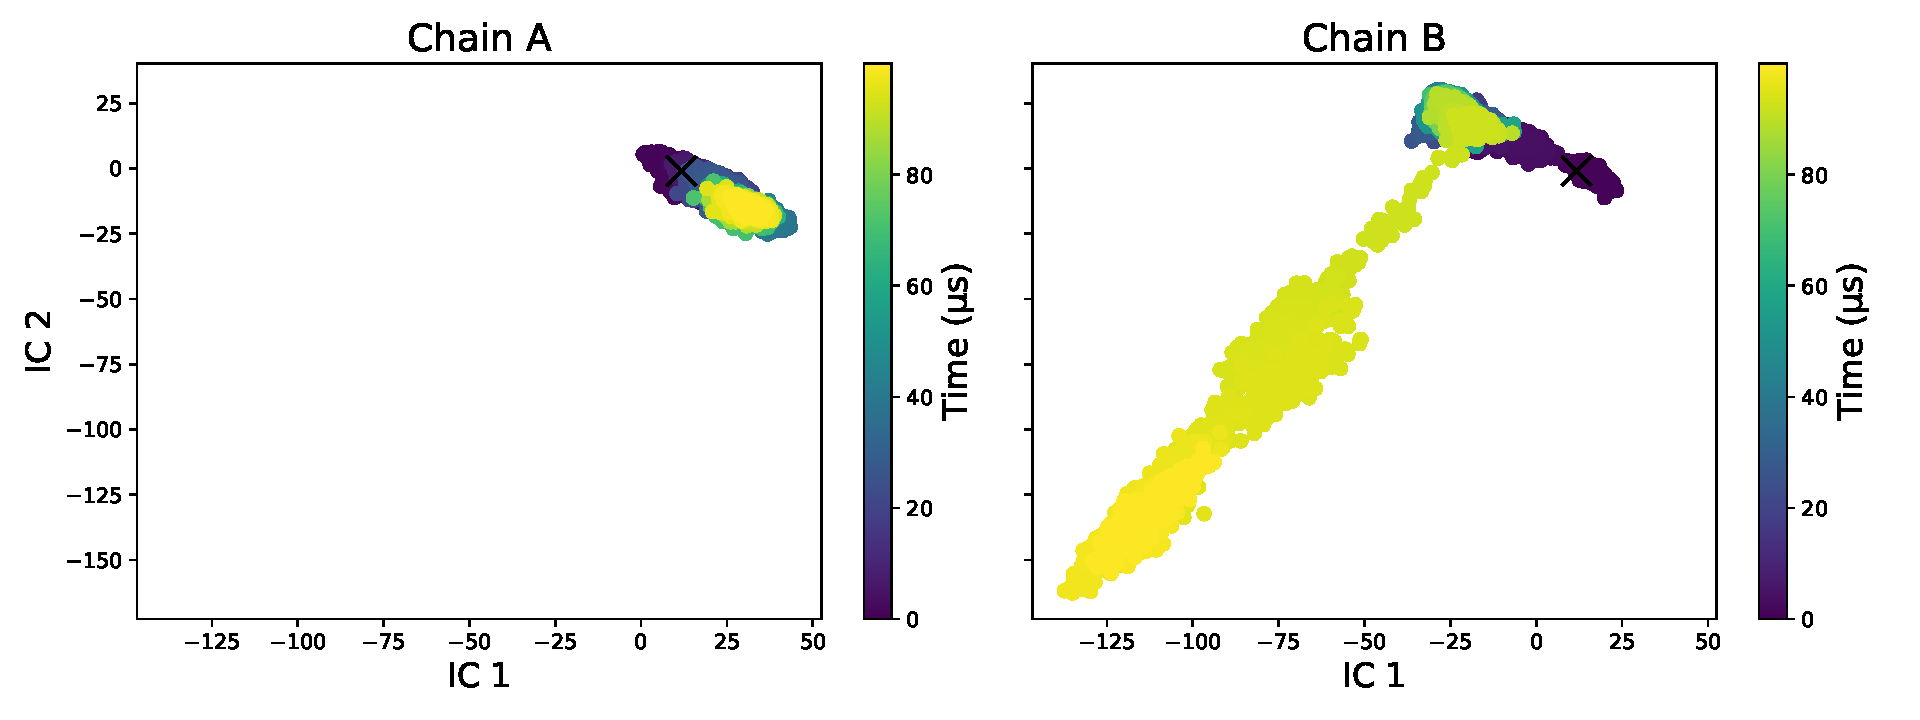
\includegraphics[width=0.6\linewidth]{fig_1_fdiscolortime_ic2.pdf}
\caption{Motions of A) monomer A and B) monomer B in Independent component 1 and 2 space colored by simulation time. Numbered points represent cluster centers}
\label{fig:view}
\end{figure}

\begin{figure}[h]
% alignment-along-ic1
\centering
\includegraphics[width=0.6\linewidth]{example-image}
\caption{Alignment of chain B A) of cluster 46 (Red), 12 (orange), and 41 (yellow) and B) of cluster 46 (red) and the starting structure (blue)}
\label{fig:view}
\end{figure}

\begin{figure}[h]
\centering
\graphicspath{ {./images/} }
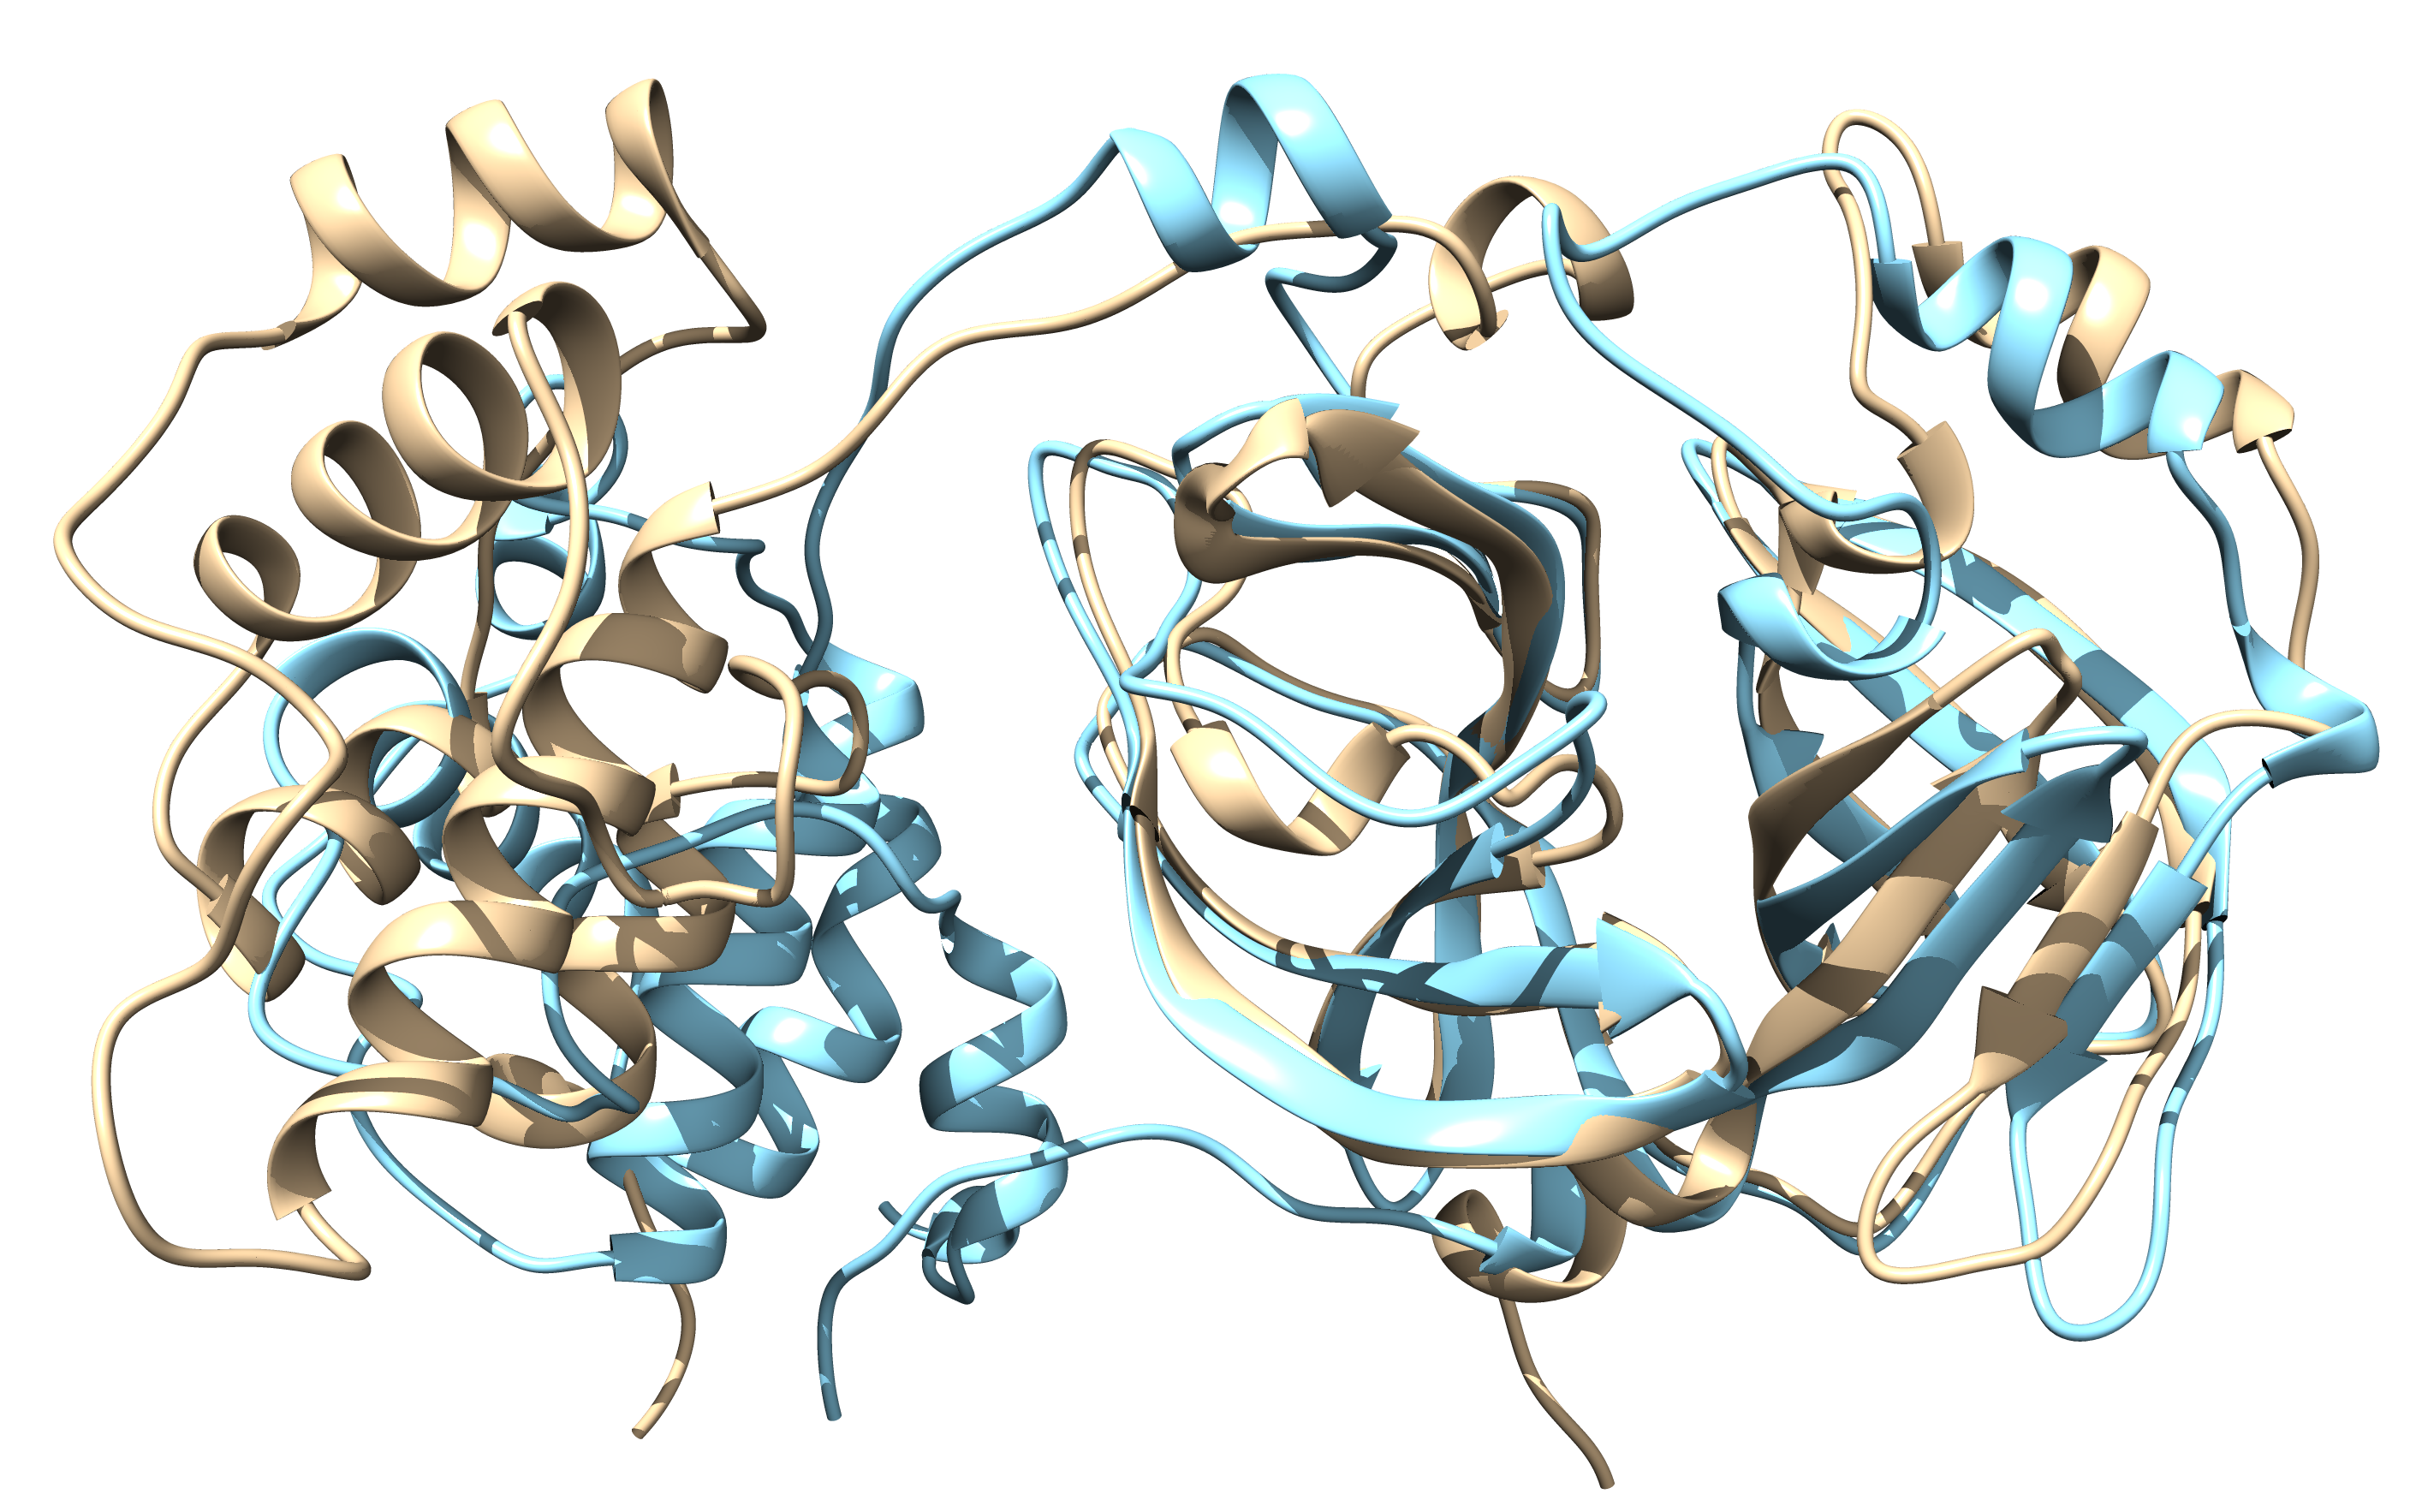
\includegraphics[width=0.6\linewidth]{blue-2Q6D-C-brown-cluster-41-better-align-2.png}
\caption{Alignment of infectious bronchitis virus, pdbid:2q6d.C (light blue) and chain B of cluster 41 (brown)}
\label{fig:view}
\end{figure}

\begin{figure}[h]
% figure made with: https://github.com/jgpattis/Desres-sars-cov-2-apo-mpro/blob/master/tica_plot_06.py
\centering
\graphicspath{ {./figures/} }
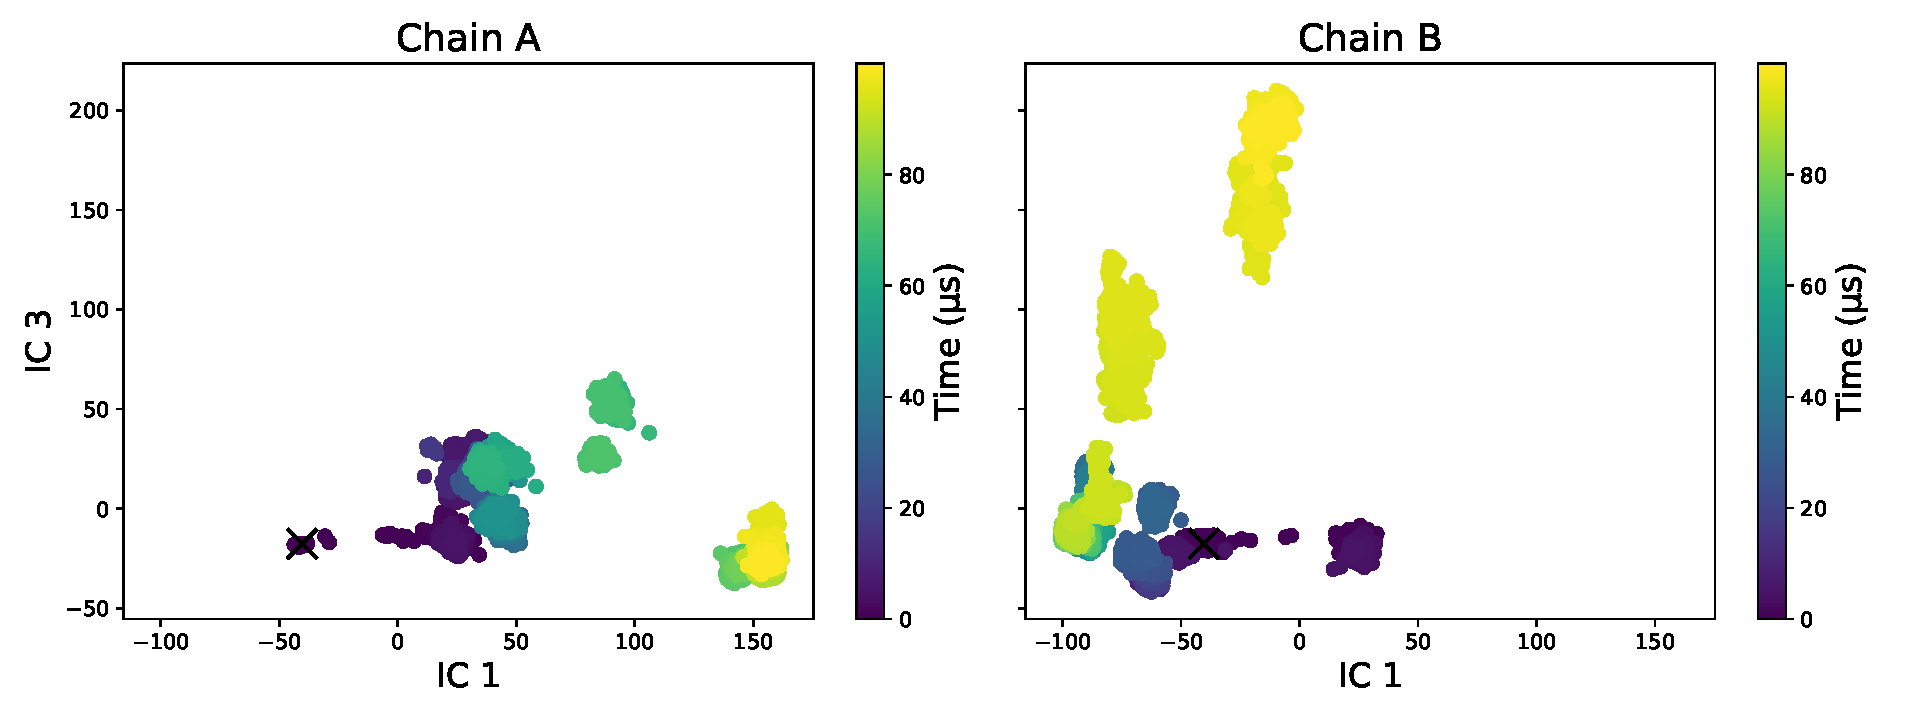
\includegraphics[width=0.6\linewidth]{fig_4_fdiscolortime_ic3.pdf}
\caption{Motions of A) monomer A and B) monomer B in Independent component 1 and 3 space colored by simulation time. Numbered points represent cluster centers}
\label{fig:view}
\end{figure}

\begin{figure}[h]
%mutual-information-heatmap
\centering
\includegraphics[width=0.6\linewidth]{example-image}
\caption{correlated motions of residue residue pairs of A) chain A and B averaged together and B) the full dimer }
\label{fig:view}
\end{figure}

\section*{Results}

\LaTeX{} is great at typesetting mathematics:

Let $X_1, X_2, \ldots, X_n$ be a sequence of independent and identically distributed random variables with $\text{E}[X_i] = \mu$ and $\text{Var}[X_i] = \sigma^2 < \infty$, and let
\begin{equation}
\label{eq:CLT}
S_n = \frac{X_1 + X_2 + \cdots + X_n}{n}
      = \frac{1}{n}\sum_{i}^{n} X_i
\end{equation}
denote their mean. Then as $n$ approaches infinity, the random variables $\sqrt{n}(S_n - \mu)$ converge in distribution to a normal $\mathcal{N}(0, \sigma^2)$. Thus concludes the explanation about Eq.~\ref{eq:CLT}.


You can make lists with automatic numbering \dots

\begin{enumerate}
\item Like this,
\item and like this.
\end{enumerate}

\dots or bullet points \dots

\begin{itemize} 
\item Like this,
\item and like this.
\end{itemize}

\dots or with words and descriptions \dots

\begin{description}
\item[Word] Definition
\item[Concept] Explanation
\item[Idea] Text
\end{description}

An example quotation:

\begin{quote}
Lorem ipsum dolor sit amet, consectetur adipiscing elit, sed do eiusmod tempor incididunt ut labore et dolore magna aliqua. Ut enim ad minim veniam, quis nostrud exercitation ullamco laboris nisi ut aliquip ex ea commodo consequat.
\end{quote}


\section*{Discussion}

\LaTeX{} formats citations and references automatically using the bibliography records in your .bib file, which you can edit via the project menu. Use the \verb|\cite| command to insert a citation, like this: \cite{Chen_Nicholson00} Multiple citations can be given as \cite{Stiles_Bartol01,el-Kareh_etal93,Callaghan91}. You can use either BibTeX or biblatex: see the following subsections.

If your manuscript is accepted, the Biophysical production team will re-format the references for publication. \emph{It is not necessary to format the reference list yourself to mirror the final published form.}

\subsection*{Using bibtex} 
This is the default. Specify your \texttt{.bib} file with \verb|\bibliography{sample}| (the extension is unnecessary) near the end of your manuscript, where you want the references list to appear.

\subsection*{Using biblatex} 
Pass the \texttt{biblatex} option to the \verb|\documentclass| declaration, then specify your \texttt{.bib} file name in the \emph{preamble}: \verb|\addbibresources{sample.bib}| (the extension is necessary). Write \verb|\printbibliography| near the end of your manuscript where you want the references to appear.

\section*{Conclusion}

Sed ut perspiciatis unde omnis iste natus error sit voluptatem accusantium doloremque laudantium, totam rem aperiam, eaque ipsa quae ab illo inventore veritatis et quasi architecto beatae vitae dicta sunt explicabo. 

\section*{Author Contributions}

Author1 designed the research. Author2 carried out all simulations, analyzed the data. Author1 and Author2 wrote the article. 

\section*{Acknowledgments}

We thank G. Harrison, B. Harper, and J. Doe for their help.

% Uncomment if using bibtex (default)
\bibliography{sample}

% Uncomment if using biblatex
% \printbibliography

\section*{Supplementary Material}

An online supplement to this article can be found by visiting BJ Online at \url{http://www.biophysj.org}.

\begin{figure}[ht]
\centering
% image made using starting structure: https://github.com/jgpattis/Desres-sars-cov-2-apo-mpro/blob/master/DESRES_protease_chainid.pdb
% and tcl file from: https://github.com/jgpattis/Desres-sars-cov-2-apo-mpro/blob/master/filter_distance_01.py
\graphicspath{ {./images/} }
% fdis-visualization.png
\includegraphics[width=0.6\linewidth]{example-image}
\caption{A visualization of the 2389 distances included in the filtered distances featurization}
\label{fig:view}
\end{figure}

\begin{figure}[h]
feature-selection
% figure created with: https://github.com/jgpattis/Desres-sars-cov-2-apo-mpro/blob/master/plot_vamp_score_04.py
\centering
\includegraphics[width=0.6\linewidth]{example-image}
\caption{The Vamp-2 score of different feature options scored on the top 10 eigenvalues of the VAMP dimentionality reduction while running 20 iterations of 50:50 shuffle split cross validation}
\label{fig:view}
\end{figure}

\begin{figure}[alignment-linker-helix]
\centering
\includegraphics[width=0.6\linewidth]{example-image}
\caption{Alignment of chain B of cluster 48 (green) and cluster 19 (iceblue)}
\label{fig:view}
\end{figure}

\begin{figure}[mutual-information-average]
\centering
\includegraphics[width=0.6\linewidth]{example-image}
\caption{visualization of residue pairs with high correlation (red lines) MI over 0.35 and moderate correlation (blue) MI over 0.15 averaged between the two chains A) AND B) rotated 180 degrees}
\label{fig:view}
\end{figure}

\begin{figure}[mutual-information-average]
\centering
\includegraphics[width=0.6\linewidth]{example-image}
\caption{visualization of residue pairs with high correlation (red lines) MI over 0.35 and moderate correlation (blue) MI over 0.15 for the dimer A) AND B) rotated 180 degrees}
\label{fig:view}
\end{figure}

\end{document}
